\documentclass{article}
\usepackage{amsmath}
\usepackage{xcolor}
\usepackage[margin=1in]{geometry}
\usepackage{graphicx}
\usepackage{mdframed}
\usepackage{float}
\usepackage{xcolor}
\usepackage{tikz}

\definecolor{solutionblue}{RGB}{0,0,255}
\usetikzlibrary{plotmarks}

\begin{document}

% Header
\begin{center}
    \textbf{\LARGE Assignment 7} \\[1ex]
    \textbf{ECE 360} \\[1ex]
    \textbf{V00984826} \\[2ex]
\end{center}

% Question and Solution Template

% Example Question and Solution (B-7-1, S-7-1)
\section*{B-7-1}

% Question text
Consider the unity-feedback system with the open-loop transfer function:
\[
G(s) = \frac{10}{s + 1}
\]
Obtain the steady-state output of the system when it is subjected to each of the following inputs:

\begin{itemize}
    \item[(a)] \( r(t) = \sin \left( t + 30^\circ \right) \)
    \item[(b)] \( r(t) = 2 \cos \left( 2t - 45^\circ \right) \)
    \item[(c)] \( r(t) = \sin \left( t + 30^\circ \right) - 2 \cos \left( 2t - 45^\circ \right) \)
\end{itemize}

% Insert question image if needed
%\begin{center}
%    \includegraphics[width=0.8\textwidth]{image_B-7-1} % Replace "image_B-7-1" with the actual filename
%\end{center}

\section*{S-7-1}

For a unity feedback system with open-loop transfer function $G(s) = \frac{10}{s + 1}$, we'll analyze the steady-state response to sinusoidal inputs.

\subsection*{Preliminary Analysis}
The closed-loop transfer function is:
\[
T(s) = \frac{C(s)}{R(s)} = \frac{G(s)}{1 + G(s)} = \frac{10}{s + 1 + 10} = \frac{10}{s + 11}
\]

For sinusoidal inputs, we utilize the frequency response approach. The general form of $T(j\omega)$ is:
\[
T(j\omega) = \frac{10}{j\omega + 11} = \frac{10}{\sqrt{\omega^2 + 121}}\angle{-\tan^{-1}\left(\frac{\omega}{11}\right)}
\]

\subsection*{Part (a): $r(t) = \sin(t + 30°)$}
\textbf{Given Input:}
\begin{itemize}
    \item Angular frequency: $\omega = 1$ rad/s
    \item Initial phase: $\theta_1 = 30°$
    \item Amplitude: $A_1 = 1$
\end{itemize}

\textbf{Analysis:}
\begin{align*}
\text{Magnitude Response:} \quad |T(j1)| &= \frac{10}{\sqrt{1^2 + 11^2}} \\
&= \frac{10}{\sqrt{122}} \\
&= 0.905
\end{align*}

\begin{align*}
\text{Phase Response:} \quad \phi_1 &= -\tan^{-1}\left(\frac{1}{11}\right) \\
&= -5.2°
\end{align*}
{\color{solutionblue}
\textbf{Steady-State Output:}
\boxed{C_{ss,a}(t) = 0.905\sin(t + 30° - 2.2°) = 0.905\sin(t + 27.8°)}}

\subsection*{Part (b): $r(t) = 2\cos(2t - 45°)$}
\textbf{Given Input:}
\begin{itemize}
    \item Angular frequency: $\omega = 2$ rad/s
    \item Initial phase: $\theta_2 = -45°$
    \item Amplitude: $A_2 = 2$
\end{itemize}

\textbf{Analysis:}
\begin{align*}
\text{Magnitude Response:} \quad |T(j2)| &= \frac{10}{\sqrt{2^2 + 11^2}} \\
&= \frac{10}{\sqrt{125}} \\
&= 0.895
\end{align*}

\begin{align*}
\text{Phase Response:} \quad \phi_2 &= -\tan^{-1}\left(\frac{2}{11}\right) \\
&= -10.3°
\end{align*}

{\color{solutionblue}\textbf{Steady-State Output:}
\boxed{C_{ss,b}(t) = 2(0.895)\cos(2t - 45° - 10.3°) = 1.79\cos(2t - 55.3°)}}

\subsection*{Part (c): $r(t) = \sin(t + 30°) - 2\cos(2t - 45°)$}
\textbf{Application of Superposition Principle:}
{Since the system is linear, we can apply the principle of superposition. The steady-state response to the combined input is the sum of the individual responses found in parts (a) and (b).}\\

{\color{solutionblue}
\textbf{Steady-State Output:}
\boxed{C_{ss,c}(t) = 0.905\sin(t + 27.8°) - 1.79\cos(2t - 55.3°)}}

\subsection*{Important Observations}
For any sinusoidal input with frequency $\omega$, the steady-state output exhibits the following characteristics:

\begin{enumerate}
    \item \textbf{Magnitude Relationship:}
    \[
    |T(j\omega)| = \frac{10}{\sqrt{\omega^2 + 121}}
    \]
    
    \item \textbf{Phase Relationship:}
    \[
    \phi(\omega) = -\tan^{-1}\left(\frac{\omega}{11}\right)
    \]
    
    \item \textbf{Output Properties:}
    \begin{itemize}
        \item Frequency remains unchanged from input to output
        \item Amplitude is scaled by $|T(j\omega)|$
        \item Phase is shifted by $\phi(\omega)$
    \end{itemize}
\end{enumerate}

%\subsection*{Verification Method}
%To verify these results, one can:
%\begin{itemize}
%    \item Substitute $t = 0$ to check initial conditions
%    \item Check that the output maintains the input frequency
%    \item Verify that amplitude ratios are correct using Bode plot principles
%    \item Confirm phase shifts using phase angle calculations
%\end{itemize}

\section*{B-7-4}
Plot the Bode diagram of 
\[
G(s) = \frac{10(s^2 + 0.4s + 1)}{s(s^2 + 0.8s + 9)}
\]

\section*{S-7-4}
The following MATLAB program produces the Bode diagram shown below.

\begin{mdframed}
{\color{solutionblue}
\begin{verbatim}
% ***** Bode diagram *****
num = [0 10 4 10];
den = [1 0.8 9 0];
bode(num, den)
title('Bode Diagram of G(s) = 10(s^2 + 0.4s + 1)/[s(s^2 + 0.8s + 9)]')
\end{verbatim}}
\end{mdframed}
\begin{figure}[H]
    \centering
    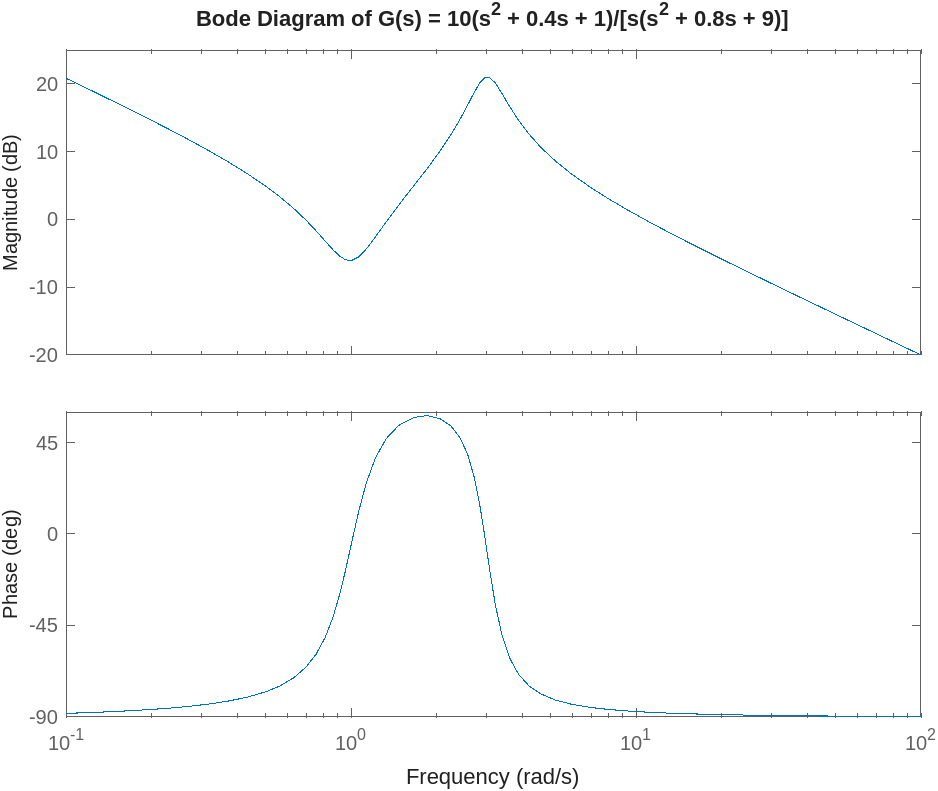
\includegraphics[width=0.85\textwidth]{/Users/arfaz/Desktop/ThirdYearEngineering/2 Fall 2024/1 ECE 360 A01 B05/1 Q-As/MatLab Files/A7/ECE360-B-7-4.png}
    \caption{Bode Diagram of \( G(s) = \frac{10(s^2 + 0.4s + 1)}{s(s^2 + 0.8s + 9)} \)}
\end{figure}

\section*{B-7-5}
Given
$ G(s) = \frac{\omega_n^2}{s^2 + 2\zeta\omega_n s + \omega_n^2} $
show that $ |G(j\omega_n)| = \frac{1}{2\zeta} $

\section*{S-7-5}
Let's solve this step by step:

\begin{enumerate}
    \item First, we substitute $s = j\omega_n$ into $G(s)$:
    \[
    G(j\omega_n) = \frac{\omega_n^2}{(j\omega_n)^2 + 2\zeta\omega_n(j\omega_n) + \omega_n^2}
    \]

    \item Simplify the denominator:
    \[
    G(j\omega_n) = \frac{\omega_n^2}{-\omega_n^2 + 2\zeta\omega_n^2j + \omega_n^2}
    \]
    \[
    = \frac{\omega_n^2}{2\zeta\omega_n^2j}
    \]
    \[
    = \frac{1}{2\zeta j}
    \]

    \item Taking the magnitude:
    \[
    |G(j\omega_n)| = \left|\frac{1}{2\zeta j}\right| = \frac{1}{|2\zeta j|} = \frac{1}{2\zeta}
    \]
\end{enumerate}
{\color{solutionblue} Therefore, we have proven that $|G(j\omega_n)| = \frac{1}{2\zeta}$}.

\section*{B-7-7}
Sketch the polar plots of the open-loop transfer function
\[
G(s)H(s) = \frac{K(T_as + 1)(T_bs + 1)}{s^2(Ts + 1)}
\]
for the following two cases:
\begin{itemize}
    \item[(a)] $T_a > T > 0$, \quad $T_b > T > 0$
    \item[(b)] $T > T_a > 0$, \quad $T > T_b > 0$
\end{itemize}

\section*{S-7-7}
The Nyquist plots for cases (a) and (b) are shown below. The key difference between the two cases lies in the relationship between the time constants, which affects the shape of the curves.

\begin{figure}[H]
    \centering
    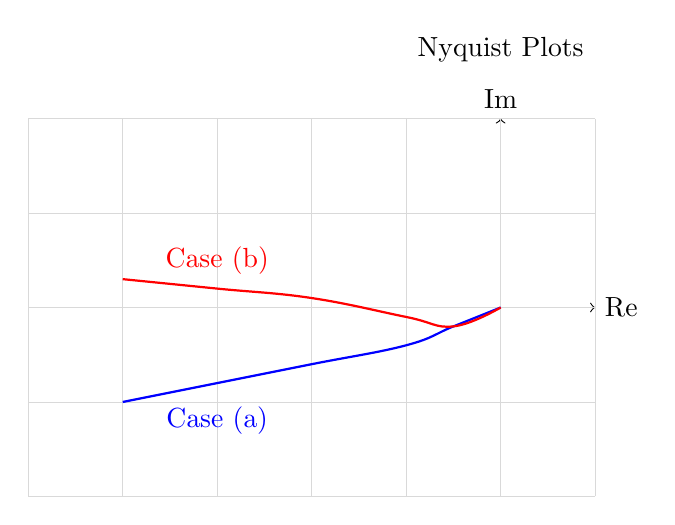
\begin{tikzpicture}[scale=1.2]
        % Draw axes
        \draw[->] (-5,0) -- (1,0) node[right] {Re};
        \draw[->] (0,-2) -- (0,2) node[above] {Im};
        
        % Draw grid
        \draw[very thin,gray!30] (-5,-2) grid (1,2);
        
        % Draw curves
        % Case (a): Ta > T > 0, Tb > T > 0
        \draw[blue, thick] plot[smooth, tension=0.7] 
            coordinates {(-4,-1) (-3,-0.8) (-2,-0.6) (-1,-0.4) (-0.5,-0.2) (0,0)};
            
        % Case (b): T > Ta > 0, T > Tb > 0
        \draw[red, thick] plot[smooth, tension=0.7] 
            coordinates {(-4,0.3) (-3,0.2) (-2,0.1) (-1,-0.1) (-0.5,-0.2) (0,0)};
            
        % Labels
        \node[blue] at (-3,-1.2) {Case (a)};
        \node[red] at (-3,0.5) {Case (b)};
        
        % Title
        \node[above] at (0,2.5) {Nyquist Plots};
    \end{tikzpicture}
    \caption{Nyquist plots for cases (a) and (b)}
\end{figure}

\textbf{Analysis of the plots:}

\begin{itemize}
    \item \textbf{Case (a)} $T_a > T > 0$, $T_b > T > 0$:
    \begin{itemize}
        \item The curve starts from the negative real axis
        \item Shows a more pronounced curvature in the lower half-plane
        \item Approaches the origin from below
    \end{itemize}
    
    \item \textbf{Case (b)} $T > T_a > 0$, $T > T_b > 0$:
    \begin{itemize}
        \item The curve starts in the upper half-plane
        \item Has a gentler curvature
        \item Crosses the real axis and approaches the origin from below
    \end{itemize}
\end{itemize}

The differences in the curves arise from how the zeros (determined by $T_a$ and $T_b$) interact with the poles (determined by $T$) in each case. In case (a), the zeros are slower than the non-zero pole, while in case (b), the zeros are faster than the non-zero pole, leading to the distinct shapes observed.

% Insert solution image if needed
%\begin{center}
%    \includegraphics[width=0.8\textwidth]{image_S-7-1} % Replace "image_S-7-1" with the actual filename
%\end{center}

% Additional Question and Solution (B-7-2, S-7-2) follow the same structure

\end{document}
